\documentclass[a4paper,12pt]{article}
\usepackage[a4paper, total={6in, 9in}]{geometry}
\usepackage{amsmath,amsfonts,euscript,times,harvard,color,fancyhdr,float}
\usepackage[backend=biblatex, bibstyle=authoryear, style=numeric,sorting=none]{biblatex}

% \usepackage[backend=biber]{biblatex-chicago}
\bibliography{bibliography}
\usepackage[pdflatex]{graphicx}
\usepackage{hyperref}
\usepackage{graphicx}

\def\RSS {{\rm RSS}}
\def\PRSS {{\rm PRSS}}
\def\bias {{\rm Bias}}
\def\ev {{\rm E}}
\def\EPE{{\rm EPE}}
\def\argmax {{\rm argmax}}
\def\Ave{{\rm Ave}}
\def\cov {{\rm Cov}}
\def\var {{\rm Var}}
\def\mse {{\rm Mse}}
\def\bX {{\bf X}}
\def\bx {{\bf x}}
\def\Pr{{\rm Pr}}
\def\bfeta{{\bf f}}
\def\bbeta{{\bf\beta}}
\def\bepsilon{{\bf \epsilon}}
\def\by{{\bf y}}
\def\bx{{\bf x}}
\def\bq{{\bf q}}
\def\bz{{\bf z}}
\def\br{{\bf r}}
\def\var { {\rm Var}\;}
\def\argmin { {\rm argmin}\;}
\def \ev {{\rm E}\;}
\def\mse{{\rm Mse}\;}
\def\ridge { {\rm ridge}}
\def\pls { {\rm pls}}
\def\pcr { {\rm pcr}}
\def\lasso { {\rm lasso}}
\def\cS{{\cal S}}
\def\bone{{\bf 1}}

\graphicspath{ {./images/} }


\title{Techniques for group-wise feature selection and estimation}
\date{}
\author{
\\
\\
Aditya Chindhade
\\ Carnegie Mellon University
\\ Master's Project Report
\\ 2018
\\
\\
\\Advisor: Prof. Nikolaos V. Sahindis 
}
\begin{document}
	\pagenumbering{gobble}
	\maketitle

	\newpage
	\tableofcontents \\
% \\ Regularization and feature selection
% \\ The ALAMO approach
% \\ Application to neural networks
% \\ Dataset description and exploration
% \\ Results
% \\ Conclusion


	\newpage
	\pagenumbering{arabic}
	\section{Abstract}
	This work presents a novel integer-programming based feature selection technique for constrained regression and comparative benchmarks with group-wise feature selection techniques. These techniques are particularly useful for incorporating prior knowledge about the structure of features in terms of hierarchy and group-wise dependence in the model building process. The uniqueness of the approach is the superior control in terms of specifying groups of features, thereby allowing the modeler to specify dependence between features and include those dependencies in the model building process. Apart from having a higher accuracy in comparison with the group-lasso, this novel approach also converges in fewer iterations. Utilizing an iterative adaptive sampling approach optimized by internal non-linear optimization solvers, this approach penalizes model complexity by using Akaike information criterion, thereby ensuring a simpler and more interpretable model while maintaining high accuracy. These capabilities have been incorporated in an integer-programming solver, ALAMO. \\
    The paper also includes benchmarks with the group-lasso penalty on a neural network to obtain sparsity in terms of hidden units, thereby incorporating structured-sparsity based regularization in a neural network. This not only solves the problem of overfitting, but also makes the network sparser, thereby making predictions faster using the sparse network. This serves as a deterministic equivalent of the dropout, allowing control on setting individual weights within a hidden layer to zero. \\
    All benchmarks are tested out on the low birth weight dataset, a popular dataset involving group-wise structure in the predictors responsible for affecting the weight of a new born child. This is primarily modeled as a regression problem.
	\newpage
	\section{Introduction}
	Some of the major challenges in machine learning approaches include overfitting, high dimensionality and lack of interpretability. The aim of regularization is to mainly to avoid overfitting and in some cases also to reduce dimensionality. Feature selection techniques aim to incorporate model interpretability by selecting predictors either based upon statistical significance or upon prior knowledge of the problem at hand. Sparsity-based regularization techniques refer to the approaches for setting the coefficients corresponding to certain predictors to exactly zero, thus providing faster computation, dimensionality reduction and improving model interpretability. \\
\\
The first regularization technique dates back to 1970, when Hoerl et.al.\cite{hoerl1970ridge} incorporated the $\ell_2$ norm to shrink the coefficients of a regression solution. 
    The Lasso\cite{tibshirani1996regression} technique was invented 1996 and became one the highest cited papers in modern statistics and machine learning. Unlike the Ridge which aims at shrinking individual coefficients in the regression problem, the lasso acts as a variable selection tool by incorporating sparsity in the model. \\ \\
The elastic net, formulated in 2005 \cite{zou2005regularization} aims at achieving a balance between the ridge and the lasso, thus doing two jobs: variable selection and shrinkage. The elastic net has quickly grown to become a popular tool in modeling financial modeling due to its unique functionality \cite{kim2014forecasting}.\\ \\
Yuan and Lin \cite{yuan2006model} invented the group-lasso technique for incorporating prior knowledge about the group-wise structure of predictors. The model has occurred multiple times in highly cited articles \cite{hastie2009unsupervised,boyd2011distributed} and has secured a unique position in the statistical machine learning community, owing to its fundamental nature and utility. The following section describes these models in further detail.   



\newpage
\section{Regularization and feature selection}
\subsection{Overview}
\subsection{The Ridge}
\begin{figure}[H]
    \centering
    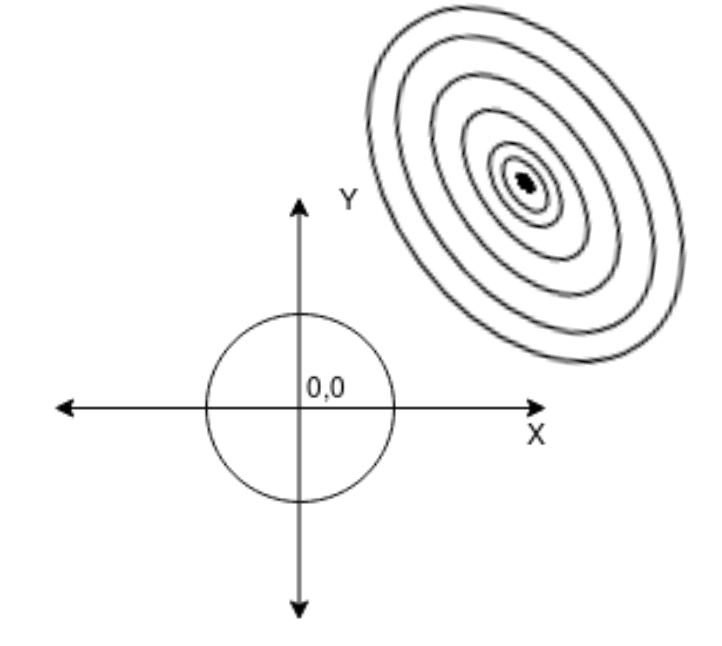
\includegraphics[scale=0.4]{ridge.png}
    \caption{The ridge penalty as a constrained minimization problem}
    \label{fig:ALAMO Flowchart}
\end{figure}
\\
The ridge utilizes the $L_2$ norm of the coefficient vector. It is responsible for shrinkage of coefficients. The degree of shrinkage is controlled by $\lambda$. It is a convex penalty and hence is tractable. The optimization problem for the ridge can be formally stated as:

\begin{eqnarray}
\label{eq:6}
\min_{\beta\in R^p}\left(||\by-\beta_0\bone-\sum_{j=1}^J
\bX_j\beta_j||_2^2 + \lambda ||\beta||_2^2 \right)
\end{eqnarray}



\newpage
\subsection{The Lasso}

\begin{figure}[H]
    \centering
    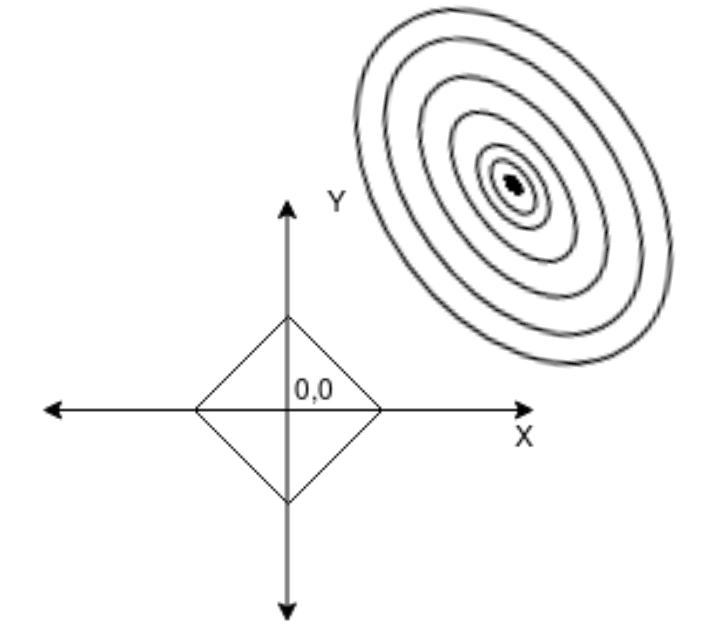
\includegraphics[scale=0.4]{lasso.png}
    \caption{The lasso penalty as a constrained minimization problem}
    \label{fig:ALAMO Flowchart}
\end{figure}
The ridge utilizes the $L_1$ norm of the coefficient vector. It is responsible for sparsity in the coefficient vector by setting coefficients to 0. The degree of sparsity is controlled by $\lambda$. Similar to the ridge, the lasso is a convex penalty and hence is tractable. The optimization problem for the ridge can be formally stated as:

\begin{eqnarray}
\label{eq:6}
\min_{\beta\in R^p}\left(||\by-\beta_0\bone-\sum_{j=1}^J
\bX_j\beta||_2^2 + \lambda ||\beta||_1 \right)
\end{eqnarray}


\newpage
\subsection{The Elastic Net}

\begin{figure}[H]
    \centering
    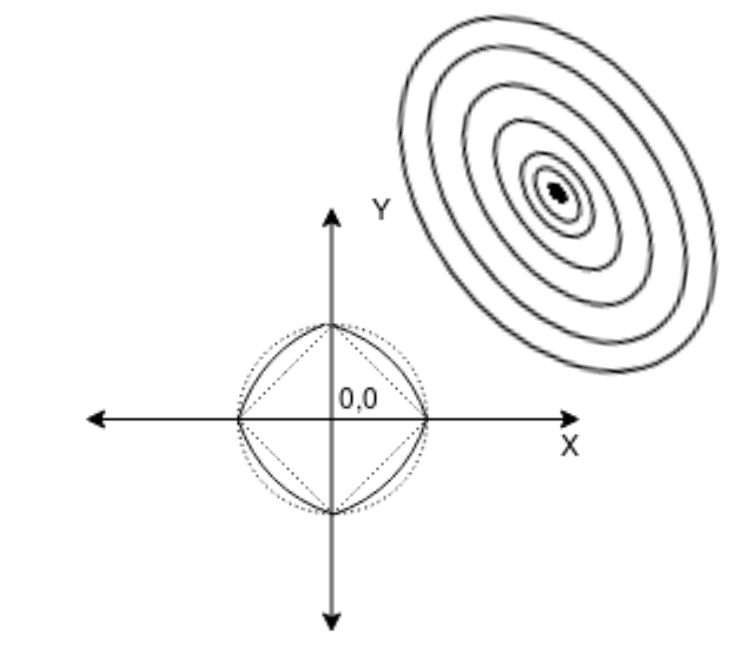
\includegraphics[scale=0.4]{elastic-net.png}
    \caption{The elastic net penalty as a constrained minimization problem}
    \label{fig:ALAMO Flowchart}
\end{figure}
The objective function for the elastic net penalized linear model is defined as:
\begin{eqnarray}
\label{eq:6}
\min_{\beta\in R^p}\left(||\by-\beta_0\bone-\sum_{j=1}^J
\bX_j\beta_j||_2^2 + \lambda_1 ||\beta||_1 + \lambda_2 ||\beta||_2^2 \right)
\end{eqnarray}
The elastic net \cite{zou2005regularization} can be considered  as an intermediate between the ridge and the lasso, addressing the shrinkage and variable selection problems simultaneously. In this representation, $\by$ is the target variable,  $\bX_\ell$ is the input matrix, $\beta_\00$  is the weight of the bias term and  $\beta_j$  is a vector corresponding to the weight of each predictor variable. $\lambda_1$ is the penalty for the  $\ell_1$ norm and $\lambda_2$  is the penalty for the $\ell_2$ norm. The relative importance of the lasso (variable selection) and the ridge (weight shrinkage) is governed by the $\lambda_1$ and $\lambda_2$ values. The requirement of two hyper-parameters can be reduced to one using a relative weight $\alpha$, given by:
$$\alpha = \frac{\lambda_2} {\lambda_1 + \lambda_2}$$
The objective function with a single hyper-parameter then becomes:
\begin{eqnarray}
\label{eq:6}
\min_{\beta\in R^p}\left(||\by-\beta_0\bone-\sum_{j=1}^J
\bX_j\beta_j||_2^2 + (1 - \alpha_1) ||\beta_j||_1 + \alpha||\beta_j||_2^2 \right)
\end{eqnarray} \\

\subsection{The Group-Lasso}

\begin{figure}[H]
    \centering
    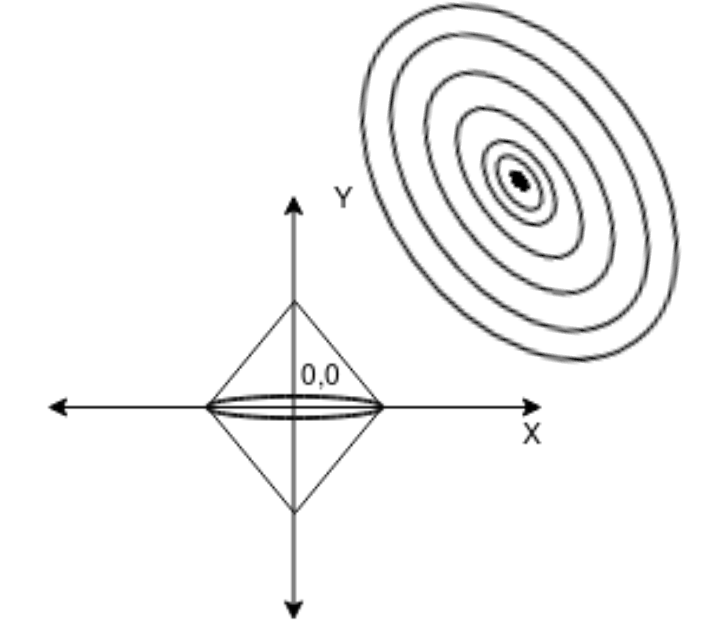
\includegraphics[scale=0.4]{group-lasso.png}
    \caption{The group lasso penalty as a constrained minimization problem}
    \label{fig:ALAMO Flowchart}
\end{figure}
Two-step penalty
Outer penalty - L1 - selecting feature groups
Inner penalty - L2 - shrinkage of coefficients within selected groups.
L+1 parameters: hyperparameters or inversely proportional to group size


The group lasso \cite{yuan2006model} penalized linear model has the following objective function:
\begin{eqnarray}
\min_{\beta\in R^p}\left(||\by-\beta_0\bone-\sum_{\ell=1}^L
\bX_\ell\beta_\ell||_2^2 +\lambda \sum_{\ell=1}^L\sqrt{p_\ell} ||\beta_\ell||_2\right)
\label{LM.grlasdef}
\end{eqnarray}
In this representation, $\by$ is the target variable,  $\bX_\ell$ is the input matrix, $\beta_\00$  is the weight of the bias term and  $\beta_\ell$  is a vector corresponding to the weight of each predictor variable across all the groups. $\lambda$ is the penalty for the group lasso and $\sqrt{p_\ell}$ is the penalty proportional to the size of each group $\ell$. This ensures  normalizing the penalty according to the size of a group. The $\ell_2$ penalty (also known as the ridge) is applied within a group to reduce the magnitude of each of the weights within a group. These norms, being positive are directly added up and effectively work as an $ \ell_1$ norm across the groups of weights.  The $ \ell_1$  norm (also known as the lasso) is responsible for selecting groups of variables and can set an entire group-wise coefficient to zero, thereby inducing sparsity in the model. \\
% The group lasso penalty is best described as a bi-pyramid structure - include diagram
\newpage
\subsection{Best subset selection}

\begin{figure}[H]
    \centering
    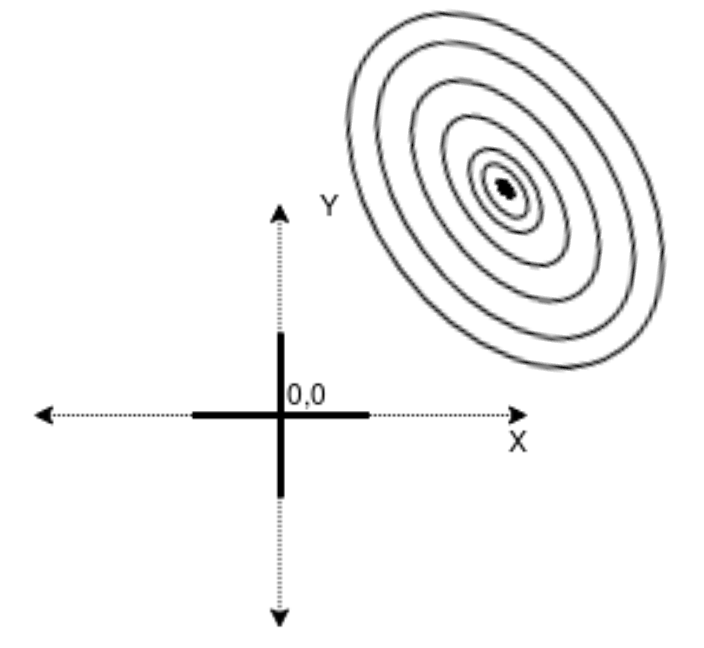
\includegraphics[scale=0.4]{best-subset.png}
    \caption{Best subset selection as a constrained minimization problem}
    \label{fig:ALAMO Flowchart}
\end{figure}

The best subset technique for feature selection is essentially an exhaustive search across all feature subsets to find the feature subset that minimizes the loss function with respect to the features vector consisting of the feature subset selected. While this isn't exactly the same as calculating a vector norm, it is known as the $L_0$ norm owing to the effective feature set obtained. Each feature can either be included in the model or excluded from it. This leads to the following relation:

\begin{eqnarray}
\textrm{Number of subsets} = 2^{\textrm{number of features}}
\end{eqnarray}
Being exponential in the number of features, the best subset selection technique is often considered intractable. However, due to the exhaustive search across feature subsets to find the best subset, this technique is widely considered as the holy grail of statistics and has been of interest lately due to advances in computing and enhancements in memory.


% \newpage
% \subsection{Summary}

% \begin{center}
% \begin{table}[]
% \begin{tabular}{|l|l|l|l|l|}
% \hline
% Technique             & Tractable & Convex & Differentiable     & Norm   \\ \hline
% Ridge                 & Yes       & Yes    & Yes                & L_2     \\ \hline
% Lasso                 & Yes       & Yes    & No                 & L_1     \\ \hline
% Elastic net           & Yes       & Yes    & Depends on penalty & L_1+L_2  \\ \hline
% Group Lasso           & Yes       & Yes    & No                 & L_1(L_2) \\ \hline
% Best subset selection & No        & No     & No                 & L_0     \\ \hline
% \end{tabular}
% \end{table}
% \end{center}

\newpage
\section{The ALAMO approach}
ALAMO \cite{cozad2014learning,cozad2015combined,wilson2017alamo} is a black-box modeling toolbox developed at the Sahinidis Optimization Group, Carnegie Mellon University. ALAMO implements an integer-programming based best-subset selection strategy for variable selection which utilizes the hallowed $\ell_0$ norm for variable selection and solves non-convex the optimization problem using derivative-free optimization solvers. The ALAMO approach relies on two key steps:

\subsection{Surrogate Model Generation}
The solution approach begins by sampling an initial set of points from the input data set, which are then used for building an initial model with, starting with the lowest complexity. Various combinations of simple basis functions are considered for generating algebraic models, which are then solved using an optimization framework. 
%write more about alamo

\subsection{Adaptive Sampling}
Adaptive sampling is an active learning \cite{angluin1988queries,settles.tr09} approach which involves querying the data for selecting the next set of points such that maximum model accuracy can be obtained with minimum additional information. This is done by an error-maximization strategy, which means that the points which have the largest deviation from the model are included in the next sample for model building. The estimate can also be made robust (insensitive to outliers) by setting a threshold on the maximum deviation allowed.   
\subsection{Constrained regression in ALAMO}
ALAMO allows manual specification of constraints on features and includes specification of feature groups. These feature groups could be defined by either polynomial transformations of the same feature forming a group or based on prior knowledge about heirarchical structure within the features. 
\begin{itemize}
    \item REQ: If group i is selected, group j is also selected.
    \item XCL: If group i is selected, group j is NOT selected and vice-versa.
    \item NMT: Not more than k variables within group i must be selected.
    \item ATL: At least k variables within group i must be selected.
\end{itemize}


\newpage

\begin{figure}[H]
 \centering
 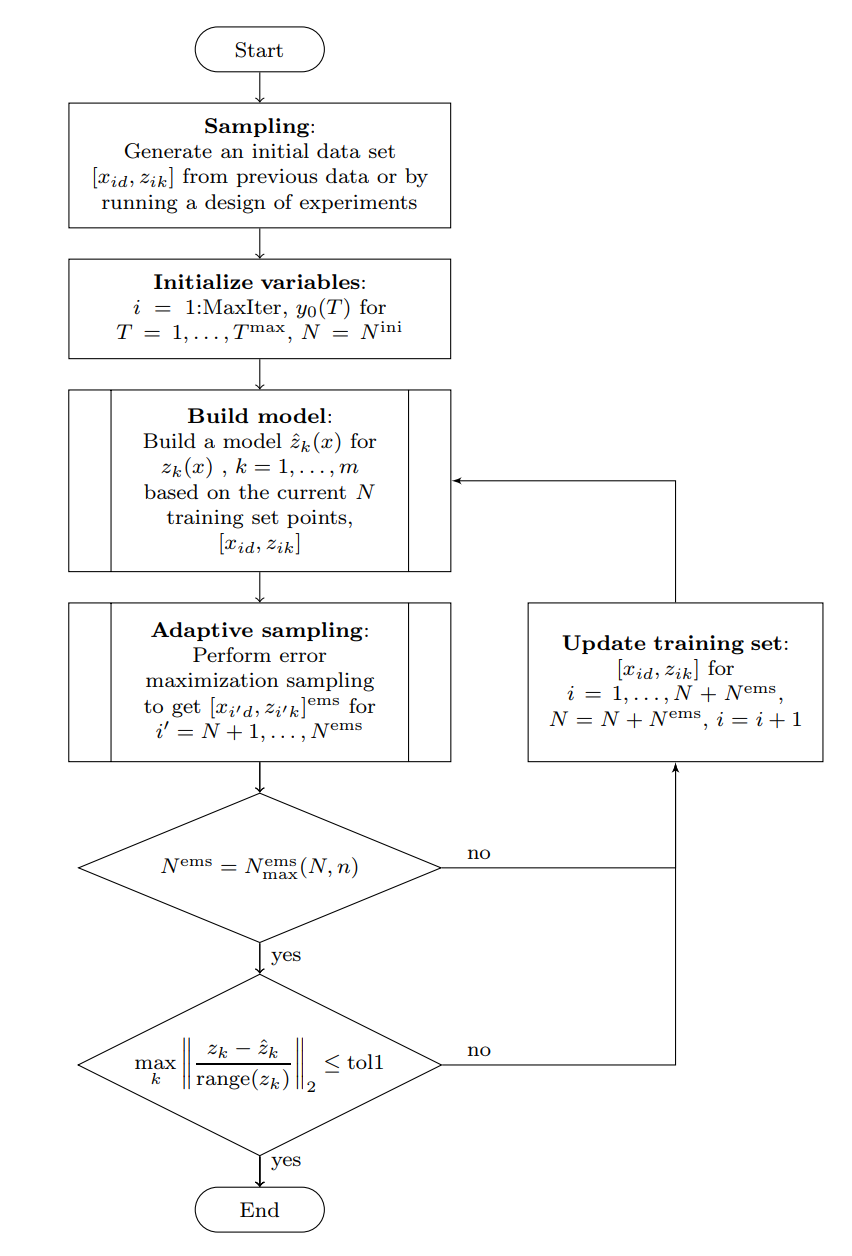
\includegraphics[scale=0.4]{flowchart-alamo.png}
 \caption{The ALAMO approach}
  \label{fig:ALAMO Flowchart}
\end{figure}

\newpage

\section{Group-sparsity in neural networks}
\subsection{Neural networks and deep learning}
Explain neural networks and their working in brief
Although neural networks were conceptualized in the mid $20^{th}$ Century, it wasn't until the recent advances in computing power that they came into vogue and remarkable accuracies\cite{lecun2015deep}were achieved due to addition of more hidden units or stacking more layers. However, the presence of too many parameters or weights quickly led to the model overfitting to the training data. To solve this problem, dropout\cite{srivastava2014dropout}, a method which involves setting neurons inactive in a stochastic manner was adopted in popular platforms. However, the inherent stochastic nature of the dropout leads to a lack of reliability and interpretability. 
\begin{figure}[H]
 \centering
 \includegraphics[scale=0.4]{nn.png}
 \caption{Neural network representation}
  \label{fig:ALAMO Flowchart}
\end{figure}

\subsection{Overfitting and regularization}
Additionally, it was proven \cite{denil2013predicting} that in most cases, only a small fraction of the learned weights contribute to the accuracy and a large number of weights can be set to zero, without significantly affecting the accuracy of the model.

\subsection{Group lasso penalty in a neural network}
More recently, group sparse regularization techniques have been applied to incorporate sparsity in the weights of a neural, thus incorporating structure in the sparsification and thereby increasing the interpretability of the model. This method serves as an additional proof to the proposition that most of the learned weights could be set to zero, by comparing accuracy with number of active neurons. \\ \\
% For example, structured sparsity can be induced in a 2x5 matrix as shown in the figure below. The gray regions represent inactive neurons (weight set to zero), while the white regions represent non-zero weights.
% In this implementation, the authors have used the group lasso penalty on the transformation of each layer in a neural network.
% The activation is given by
% image.png where { Wk , bk } are the parameters of the layer, while gk ( ·) is the activation function to be applied element-wise.
% The optimal value of Wk is given by:
% image.png where L is a loss function and R is a regularization function.
% The regularization function for the group lasso is given by:
% image.png
% We need a group-lasso penalty to ensure that all outputs from this layer are set to 0. If this layer happens to be the input layer, it means that this particular feature is not selected. Taking an example of a 2x5 weight matrix (2 input units and 5 hidden units), the sparsity can be seen as follows:
% image.png

% The white regions correspond to non-zero weights while the grey regions correspond to the weights that have been set to 0. Using this form of group-regularization, the authors obtained the following results:

% image.png
% image.png

% It can be seen that if the penalty is below 10\^-3, the accuracy is pretty much the same as that without the group lasso penalty. However, the sparsity induced is significant. For example, the features can be reduced from 64 (8x8 image) to 48, without affecting the accuracy significantly.


\newpage
\section{Experiments}
	\subsection{Dataset description}
		The data-set under consideration was first published in a book - Applied Logistic Regression by Hosmer and Lemeshow \cite{hosmer2013applied} and consists of the  data were collected at Baystate Medical Center, Springfield, Mass during 1986. The data in the raw format can be found in popular repositories like MLData (http://www.mldata.org/repository/data/viewslug/uci-20070111-lowbwt/). Basic transformations on the features lead to the following features:
    

\item age1,age2,age3:Orthogonal polynomials of first, second, and third degree representing mother’s age in years (float)
\item lwt1,lwt2,lwt3:Orthogonal polynomials of first, second, and third degree representing mother’s weight in pounds at last menstrual period (float)
\item white,black:Indicator functions for mother’s race; "other" is reference group (boolean)
\item smoke:Smoking status during pregnancy (boolean)
\item ptl1,ptl2m:Indicator functions for one or for two or more previous premature labors, respectively. No previous premature labors is the reference category. (integer)
\item ht:History of hypertension (boolean)
\item ui:Presence of uterine irritability (boolean)
\item ftv1,ftv2,ftv3m:Indicator functions for one, for two, or for three or more physician visits during the first trimester, respectively. No visits is the reference category. (boolean)

\end{itemize}
\subsection{Feature transformations}
        Additional features corresponding to polynomial transformations
        One-hot encoding for categorical features
        Mean-normalization for continuous 
        
        Feature groups are identified based on either polynomial transformations of the same primary variable or prior knowledge about association
        \begin{figure}[H]
     \centering
     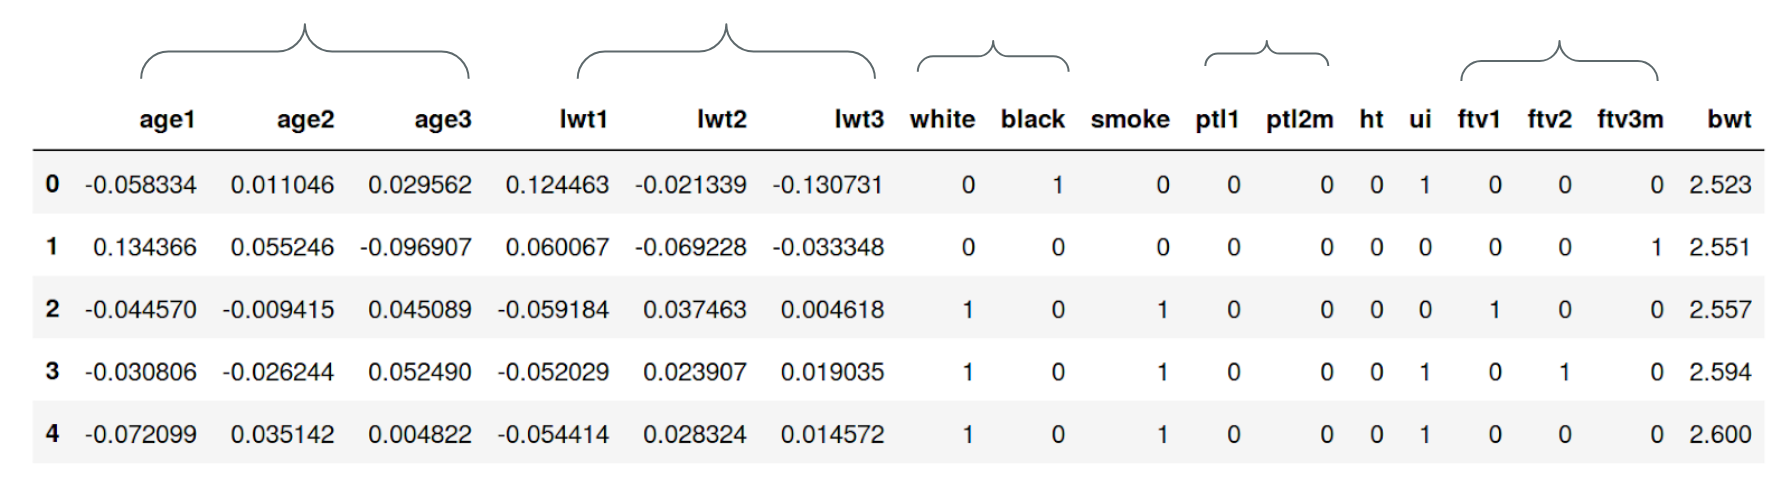
\includegraphics[scale=0.25]{feature-grouping.png}
     \caption{Identification of feature groups}
      \label{fig:ALAMO Flowchart}
    \end{figure}

        
        
\subsection{Correlation plot}
    \begin{figure}[H]
     \centering
     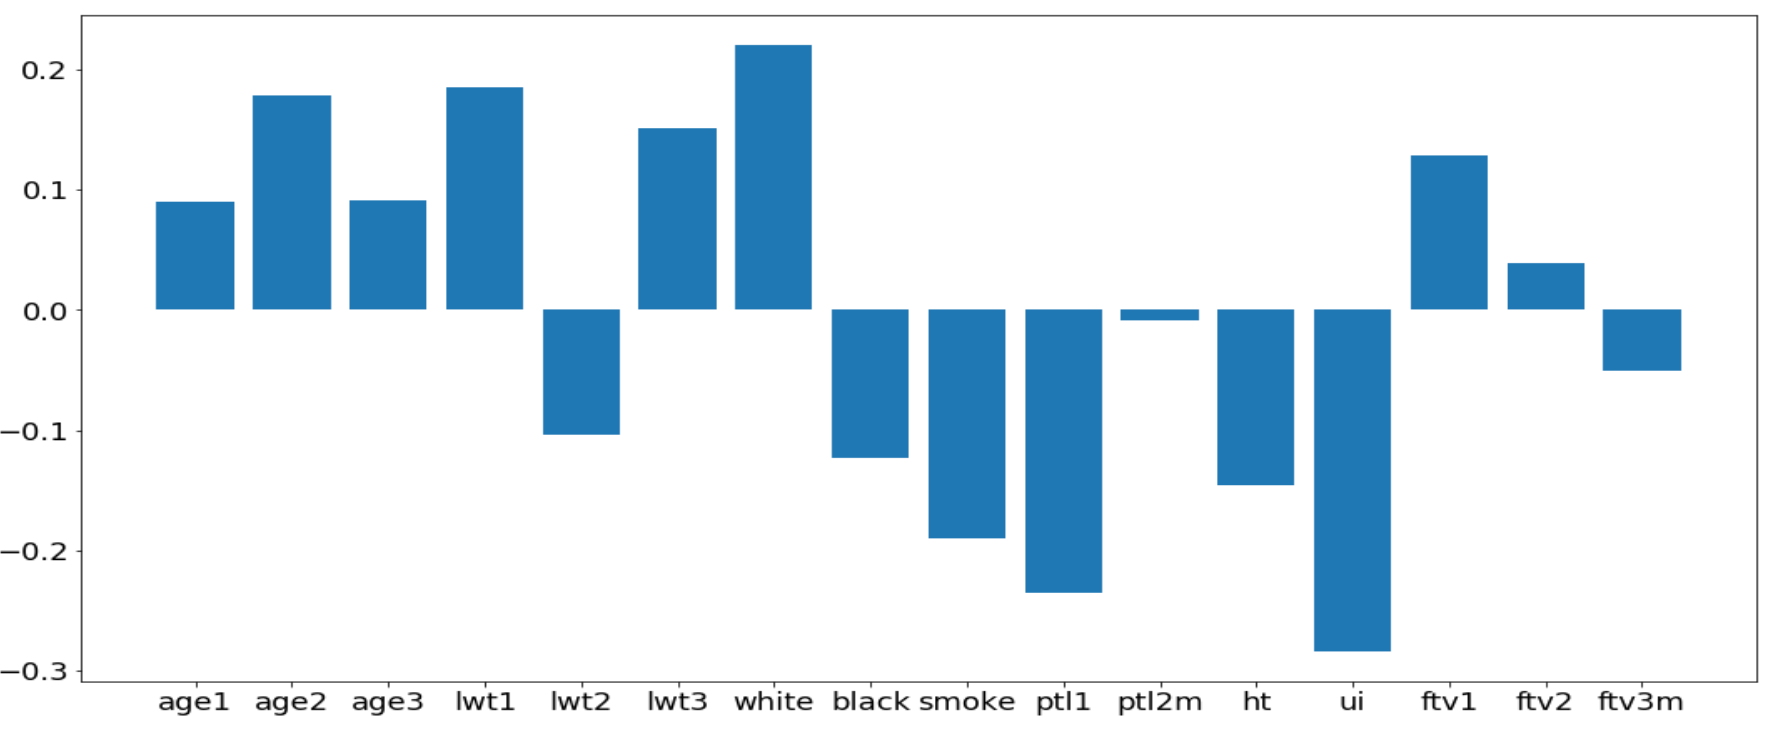
\includegraphics[scale=0.25]{corr.png}
     \caption{Correlation plot: Pearson correlation of each feature with target variable}
      \label{fig:ALAMO Flowchart}
    \end{figure}

\subsection{Modeling}
    The following models were used for fitting the data and identifying which features were selected
    % \subsubsection{Ridge}
    % The Ridge was implemented using the Sci-kit learn framework in Python.
    % \subsubsection{Lasso}
    % The Lasso was implemented using the Sci-kit learn framework in Python.
    \subsubsection{Elastic Net}
    The Elastic Net was implemented using the glmnet framework in R.
    \subsubsection{Group Lasso}
    The Group Lasso was implemented using the grpreg framework in R.
    \subsubsection{ALAMO}
    ALAMO version 2018.6.20 was downloaded from The Optimization Firm website: \href{https://minlp.com/alamo}{www.minlp.com}
    \subsubsection{Group-sparse neural network}
    The group lasso was implemented in a neural network using the source code by \cite{scardapane2017group} and a 4 layer deep neural network was built using Keras with Tensorflow backend.
    

    
	\newpage
	\section{Results and Discussion}
	\subsection{Elastic Net}
Elastic net regularization is implemented using the 'glmnet' package in R. The elastic net penalty, by nature, does not account for group-wise variable selection. As a result, sparsity can be observed in the model, however, the sparsity is unstructured and does not take into account the group-wise structure of the predictors. The sparsity pattern can be observed as follows:\\
\begin{table}[H]
\resizebox{\columnwidth}{!}{%
\begin{tabular}{|l|l|l|l|l|l|l|}
\hline
\textbf{Penalty}     & 0.01               & 0.05                & 0.1                 & 0.2                 & 0.5             & 1               \\ \hline
(Intercept) & 3.04399682125432   & 2.99862111924456    & 2.97451861554578    & 2.94729609773121    & 2.9445873015873 & 2.9445873015873 \\ \hline
age1        & 0                  & 0                   & 0                   & 0                   & 0               & 0               \\ \hline
age2        & 1.44051051842287   & 0.893538133354436   & 0.305271674803786   & 0                   & 0               & 0               \\ \hline
age3        & 0.78086581048347   & 0.277461839300162   & 0                   & 0                   & 0               & 0               \\ \hline
lwt1        & 1.72064278608912   & 0.922138791531523   & 0.188841821495976   & 0                   & 0               & 0               \\ \hline
lwt2        & 0                  & 0                   & 0                   & 0                   & 0               & 0               \\ \hline
lwt3        & 1.23031669045937   & 0.643316528641855   & 0.0127156281429045  & 0                   & 0               & 0               \\ \hline
white       & 0.283580137772934  & 0.240028719523993   & 0.1315299109623     & 0                   & 0               & 0               \\ \hline
black       & -0.128034497587724 & -0.0156065518331853 & 0                   & 0                   & 0               & 0               \\ \hline
smoke       & -0.264225200231336 & -0.198028390816008  & -0.0912396753272265 & 0                   & 0               & 0               \\ \hline
ptl1        & -0.284813413430795 & -0.225704188508818  & -0.14210767582366   & 0                   & 0               & 0               \\ \hline
ptl2m       & 0.153956928628921  & 0                   & 0                   & 0                   & 0               & 0               \\ \hline
ht          & -0.516322737244609 & -0.306829255474887  & -0.0545396147704061 & 0                   & 0               & 0               \\ \hline
ui          & -0.452482179034149 & -0.360364466248038  & -0.266681936403788  & -0.0182843739713636 & 0               & 0               \\ \hline
ftv1        & 0.0696453392572871 & 0.0211442404548328  & 0                   & 0                   & 0               & 0               \\ \hline
ftv2        & 0                  & 0                   & 0                   & 0                   & 0               & 0               \\ \hline
ftv3m       & -0.135558951958573 & 0                   & 0                   & 0                   & 0               & 0               \\ \hline
\end{tabular}
}
\caption{Sparsity pattern for the elastic net}
\end{table}
From the sparsity pattern of the elastic net penalized linear model and from the correlation plot in the previous section, it can be seen that the coefficients that are set to 0 are the ones which are least correlated with the target variable. At low values of $\lambda$, the least correlated features are set to 0. However, as the value of $\lambda$ increases, more and more coefficients are set to 0 and the order in which this is done is governed by the correlation of the feature with the target variable. 
\newpage
		\subsection{Group Lasso}
Upon running a sweep across different group-regularization penalty values from 0.01 to 0.19, it is found that as the penalty goes on increasing, the group-lasso excludes more and more groups from the model, thus inducing more sparsity in the model. \\
It was also observed that as more and more groups are excluded from the model, the MSE goes on increasing, due to an increase in the bias. \\
\\
\begin{figure}[H]
 \centering
 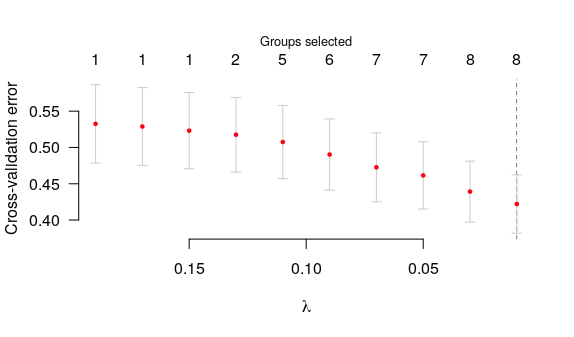
\includegraphics[scale=0.8]{err-lambda.png}
  \caption{Cross-validation error vs penalty}
  \label{fig:neurons}
\end{figure}
A trade-off between MSE and model interpretability is important. For example, the lowest MSE occurs when all 8 groups are selected, which means that unwanted predictors such as {number of physician visits} influence the output {weight of the child}. Hence, we settle for 7 groups, although it gives a slightly higher MSE than that with 8 groups. This occurs at a penalty value of 0.04. With 7 groups, we get an MSE of 0.44, which is comparable to the one found in the original group lasso paper. 

 \newpage
 The following table demonstrates the group-wise sparsity induced in the model: \\ 
\begin{table}[H]
\resizebox{\columnwidth}{!}{%
\begin{tabular}{|l|l|l|l|l|l|l|l|l|l|l|l|}
\hline
% \multicolumn{1}{|r|}{} 
\textbf{Penalty}  & 0.01    & 0.03    & 0.04    & 0.05    & 0.07    & 0.09    & 0.11    & 0.13    & 0.15    & 0.17    & 0.19    \\ \hline
(Intercept)            & 3.0434  & 3.0369  & 3.0349  & 3.0289  & 3.0176  & 3.0073  & 2.9964  & 2.9794  & 2.9681  & 2.9598  & 2.9515  \\ \hline
age1                   & 0.0055  & 0.1225  & 0.1450  & 0.1407  & 0.0824  & 0       & 0       & 0       & 0       & 0       & 0       \\ \hline
age2                   & 1.3883  & 0.9979  & 0.8113  & 0.6259  & 0.2669  & 0       & 0       & 0       & 0       & 0       & 0       \\ \hline
age3                   & 0.8102  & 0.6025  & 0.4936  & 0.3767  & 0.1568  & 0       & 0       & 0       & 0       & 0       & 0       \\ \hline
lwt1                   & 1.6682  & 1.1717  & 0.9478  & 0.7468  & 0.3743  & 0.0342  & 0       & 0       & 0       & 0       & 0       \\ \hline
lwt2                   & -0.0180 & -0.1336 & -0.1576 & -0.1584 & -0.1137 & -0.0134 & 0       & 0       & 0       & 0       & 0       \\ \hline
lwt3                   & 1.2186  & 0.8884  & 0.7292  & 0.5828  & 0.2969  & 0.0273  & 0       & 0       & 0       & 0       & 0       \\ \hline
white                  & 0.2732  & 0.2308  & 0.2093  & 0.1835  & 0.1328  & 0.0817  & 0.0217  & 0       & 0       & 0       & 0       \\ \hline
black                  & -0.1337 & -0.0916 & -0.0746 & -0.0610 & -0.0382 & -0.0207 & -0.0064 & 0       & 0       & 0       & 0       \\ \hline
smoke                  & -0.2634 & -0.2277 & -0.2101 & -0.1878 & -0.1453 & -0.1040 & -0.0531 & -0.0077 & 0       & 0       & 0       \\ \hline
ptl1                   & -0.2736 & -0.2265 & -0.1997 & -0.1742 & -0.1190 & -0.0598 & -0.0004 & 0       & 0       & 0       & 0       \\ \hline
ptl2m                  & 0.1840  & 0.1105  & 0.0817  & 0.0570  & 0.0224  & 0.0044  & 0.0000  & 0       & 0       & 0       & 0       \\ \hline
ht                     & -0.5108 & -0.4015 & -0.3493 & -0.2977 & -0.1982 & -0.1023 & -0.0223 & 0       & 0       & 0       & 0       \\ \hline
ui                     & -0.4586 & -0.4174 & -0.3988 & -0.3805 & -0.3466 & -0.3153 & -0.2678 & -0.2147 & -0.1590 & -0.1027 & -0.0464 \\ \hline
ftv1                   & 0.0688  & 0.0211  & 0       & 0       & 0       & 0       & 0       & 0       & 0       & 0       & 0       \\ \hline
ftv2                   & 0.0215  & 0.0081  & 0       & 0       & 0       & 0       & 0       & 0       & 0       & 0       & 0       \\ \hline
ftv3m                  & -0.1159 & -0.0268 & 0       & 0       & 0       & 0       & 0       & 0       & 0       & 0       & 0       \\ \hline
\end{tabular}
}
\caption{Sparsity pattern for the group lasso}

\end{table}

The sparsity pattern upon mean-normalization of the data can be seen as follows: \\
\begin{table}[H]
\resizebox{\columnwidth}{!}{%
\begin{tabular}{|l|l|l|l|l|l|l|l|l|l|l|l|}
\hline
Penalty     & 0.000000  & 0.001000  & 0.002000  & 0.003000  & 0.004000  & 0.005000  & 0.006000  & 0.007000  & 0.008000  & 0.009000  & 0.010000  \\ \hline
(Intercept) & 0.408308  & 0.407470  & 0.406824  & 0.408491  & 0.413713  & 0.419661  & 0.425577  & 0.431550  & 0.437533  & 0.442420  & 0.447314  \\ \hline
V1          & -0.050094 & -0.045197 & -0.040482 & -0.035889 & -0.032678 & -0.029972 & -0.027733 & -0.025572 & -0.023512 & -0.022112 & -0.020708 \\ \hline
V2          & -0.142799 & -0.137403 & -0.131842 & -0.125891 & -0.120009 & -0.114354 & -0.108833 & -0.103255 & -0.097624 & -0.092039 & -0.086413 \\ \hline
V3          & -0.162437 & -0.154920 & -0.147381 & -0.140226 & -0.132939 & -0.125760 & -0.118750 & -0.111769 & -0.104824 & -0.098055 & -0.091343 \\ \hline
V4          & 0.016164  & 0.010402  & 0.004833  & 0.000000  & 0.000000  & 0.000000  & 0.000000  & 0.000000  & 0.000000  & 0.000000  & 0.000000  \\ \hline
V5          & -0.003375 & -0.002185 & -0.001065 & 0.000000  & 0.000000  & 0.000000  & 0.000000  & 0.000000  & 0.000000  & 0.000000  & 0.000000  \\ \hline
V6          & 0.004636  & 0.003334  & 0.001751  & 0.000000  & 0.000000  & 0.000000  & 0.000000  & 0.000000  & 0.000000  & 0.000000  & 0.000000  \\ \hline
V7          & 0.012781  & 0.010961  & 0.009152  & 0.007400  & 0.005382  & 0.003669  & 0.002398  & 0.001159  & 0.000000  & 0.000000  & 0.000000  \\ \hline
V8          & -0.005466 & -0.004499 & -0.003591 & -0.002819 & -0.002523 & -0.002011 & -0.001383 & -0.000703 & 0.000000  & 0.000000  & 0.000000  \\ \hline
V9          & -0.008701 & -0.006843 & -0.005014 & -0.003258 & -0.001283 & 0.000000  & 0.000000  & 0.000000  & 0.000000  & 0.000000  & 0.000000  \\ \hline
V10         & 0.003976  & 0.003415  & 0.002866  & 0.002194  & 0.001580  & 0.001123  & 0.000975  & 0.000843  & 0.000729  & 0.000727  & 0.000719  \\ \hline
V11         & 0.095628  & 0.091209  & 0.086667  & 0.081750  & 0.077499  & 0.073443  & 0.069734  & 0.066031  & 0.062324  & 0.058339  & 0.054358  \\ \hline
V12         & 0.003376  & 0.001643  & 0.000000  & 0.000000  & 0.000000  & 0.000000  & 0.000000  & 0.000000  & 0.000000  & 0.000000  & 0.000000  \\ \hline
V13         & 0.003473  & 0.001552  & 0.000000  & 0.000000  & 0.000000  & 0.000000  & 0.000000  & 0.000000  & 0.000000  & 0.000000  & 0.000000  \\ \hline
V14         & 0.003564  & 0.002546  & 0.001467  & 0.000347  & 0.000000  & 0.000000  & 0.000000  & 0.000000  & 0.000000  & 0.000000  & 0.000000  \\ \hline
V15         & -0.001652 & -0.001033 & -0.000506 & -0.000090 & 0.000000  & 0.000000  & 0.000000  & 0.000000  & 0.000000  & 0.000000  & 0.000000  \\ \hline
V16         & 0.010427  & 0.007143  & 0.003934  & 0.000870  & 0.000000  & 0.000000  & 0.000000  & 0.000000  & 0.000000  & 0.000000  & 0.000000  \\ \hline
errors      & 0.036471  & 0.034605  & 0.033251  & 0.032387  & 0.031968  & 0.031590  & 0.031285  & 0.031017  & 0.030780  & 0.030574  & 0.030401  \\ \hline
\end{tabular}
}
\caption{Sparsity pattern of the elastic net upon mean-normalization}

\end{table} \\
It can be observed that the penalties have reduced by an order of magnitude to achieve the same level of sparsity in the model. This is due to the reduction in magnitude of the elements of the decision matrix.

\newpage

\newpage
\subsection{ALAMO}
Upon running the same experiment with ALAMO, with the constraints that the groups exist as specified in the R program, with an ATLEAST requirement on all groups except the {number of physician visits}. ALAMO, too, excludes this group from the model when the ATL constraint is excludes for this particular group. \\ \\
Additionally, it is observed that ALAMO gave a slightly better MSE of 0.402 as compared to 0.44 with 'grpreg' in R. Both are run on 4-fold cross-validations. The weights learned by ALAMO are also quite different from those learned by grpreg. \\
% Please add the following required packages to your document preamble:
% \usepackage{graphicx}
\begin{table}[H]
\centering
\resizebox{\textwidth}{!}{%
\begin{tabular}{|l|l|}
\hline
Model                                                          & MSE    \\ \hline
(age1, age2, age3, lwt1, lwt2, lwt3, white)                    & 0.559  \\ \hline
(age1, age2, age3, lwt1, lwt2, lwt3, white,1)                  & 0.0733 \\ \hline
(age1, age2, age3, lwt1, lwt2, lwt3, white, ui, 1)             & 0.0684 \\ \hline
(age1, age2, age3, lwt1, lwt2, lwt3, white, ht,  ui, 1)        & 0.0646 \\ \hline
(age1, age2, age3, lwt1, lwt2, lwt3, white, smoke, ht,  ui, 1) & 0.0614 \\ \hline
\end{tabular}%
}
\caption{Solution paths of ALAMO}

\end{table}
\\
The linear model can be found to be as follows:\\
Y (estimate) = - 0.30 * age1 + 0.46 * age2 + 0.35 * age3 + 0.63 * lwt1 + 0.16 * lwt2 + 0.42 * lwt3 + 0.15 * white - 0.13 * smoke - 0.26 * ht - 0.22 * ui + 1.1
\\
\\
An interesting observation is that in case of log-transformation, ALAMO selects the same model with or without specifying the group constraints.
As is evident from both instances, both models leave out ftv from the regression, but ALAMO has a slightly better accuracy as compared to the group lasso.

\newpage
\subsection{Group-lasso penalized neural network}
A feed-forward neural network with 4 layers was implemented using Keras with TensorFlow backend and the L21 (group lasso) penalty as specified in \cite{scardapane2017group}.
While the penalty doesn't allow for a manual specification of groups, it is interesting to see how the network gets sparser, while maintaining the accuracy. The neurons whose weights have been set to 0 by the group lasso penalty are defined as 'inactive' neurons. The following plot shows the active neurons vs training epochs.

A 4-fold cross validation resulted in a mean squared loss of 0.02541.
\begin{figure}[H]
 \centering
 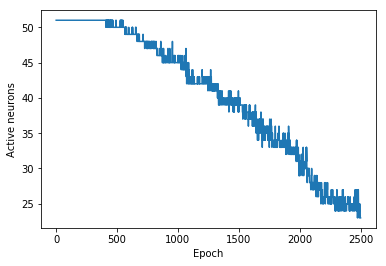
\includegraphics[scale=0.7]{nn-sparse.png}
  \caption{Number of active neurons vs epochs}
  \label{fig:neurons}
  
  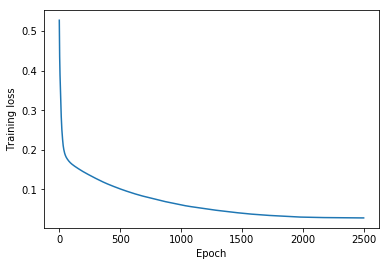
\includegraphics[scale=0.7]{loss.png}
  \caption{Mean-square error vs epochs}
  \label{fig:neurons}
\end{figure}

% \begin{figure}[H]
%  \centering
%  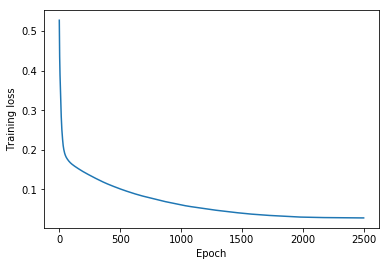
\includegraphics[scale=0.7]{loss.png}
%   \caption{Mean-square error vs epochs}
%   \label{fig:neurons}
% \end{figure}


\newpage
\section{Conclusion}
The following table summarizes the results from the 4 approaches on the raw data and on mean-normalized data:\\
\begin{table}[H]
\begin{tabular}{|l|l|l|l|1|}
\hline
& MSE on Raw data & MSE (normalized) &  Runtime (s) & Model size\\ \hline
Group-lasso                                                           & 0.441           & 0.032387  & 3.86	&11                  \\ \hline
ALAMO                                                                 & 0.402           & 0.06359   & 11.3	&11                  \\ \hline
\begin{tabular}[c]{@{}l@{}}Group-sparse\\ Neural Network\end{tabular} & 0.386           & 0.02541   & 115.018    & -            \\ \hline
\end{tabular}
\end{table}

The runtimes reported above have been calculated on a dataset with 100,000 data points and 16 features. The number of epochs for the neural network were brought down to 10 for achieving comparable runtimes. It is worth noting that upon performing performing mean-normalization of the data, the mean-squared error goes down by an order of magnitude. \\
\\The elastic net serves as an intermediate penalty between the lasso and the ridge and accounts for variable shrinkage and selection. However, it does not allow for incorporation of prior knowledge about the group-wise nature of predictors. \\The motivation for incorporating a group lasso penalty in neural networks is to reduce the dimensionality of the input space, thus reducing overall model size by setting to 0 the corresponding coefficients in the weight matrices of the consequent layers. This results in an overall sparser model, which has the advantages of fast calculations.
The motivation is akin to that of the dropout \autocite{srivastava2014dropout}, one of the most highly cited papers in deep learning.  This has tremendous applications in cases where pre-trained networks are required for fast classification (e.g. self-driving cars).\\\\
All models discussed above have their unique characteristics. The group lasso incorporates structured sparsity and allows for variable and group specification. However, the variable selection is done entirely by the tool as it learns the weights from data. ALAMO, on the other hand, allows for manual specification on the group-wise structure of predictors and also accounts for constraints on the presence and absence of certain groups of variables in the model. It also allows for non-linear transformations of the predictors, allowing for learning more complex functions from data. ALAMO also has a better cross-validation accuracy as compared to the group lasso. However, model building in ALAMO is slightly slower that the group-lasso due the non-convex nature of the $L_0$ penalty that ALAMO tries to solve and the iterative nature of the branch and bound algorithm that it utilizes. In conclusion, ALAMO provides a higher control over the model and allows for building a simpler and in consequence, a more interpretable model within comparable runtimes.

\newpage
% \nocite{*}

% \bibliography{bibliography} 
% \bibliographystyle{ieeetr}
\bibliographystyle{ieeetr}
\printbibliography

\end{document}
